\section{БиДиСек ХХК танилцуулга}
“БиДиСЕК ҮЦК” ХК нь Монгол Улсад өмч хувьчлал явагдаж Хөрөнгийн зах зээлийн харилцаа бий болсон цагаас үүсгэн байгуулагдаж өнөөг хүртэл 31 жилийн турш тасралтгүй үйл ажиллагаа явуулж буй, салбартаа тэргүүлэгч үнэт цаасны компани юм. \par
Компани нь 2006 онд Монголын Хөрөнгийн Бирж дээр IPO хийснээр нийтэд үнэт цаасаа нээлттэй санал болгосон хамгийн анхны үнэт цаасны компани болсон. \par
БиДиСЕК ҮЦК ХК нь Санхүүгийн Зохицуулах Хорооноос олгосон Андеррайтер, Брокер Дилер, Хөрөнгө оруулалтын зөвлөхийн үйлчилгээ эрхлэх тусгай зөвшөөрлийн хүрээнд үйл ажиллагаа явуулдаг бөгөөд 2017 онд гадаад улсын үнэт цаасны зах зээлд үнэт цаас худалдах, худалдан авахад зуучлах тусгай зөвшөөрөл авснаар үнэт цаасны зах зээлийн цогц үйлчилгээг харилцагчиддаа санал болгон ажиллаж байна. \par
Компани нь үйл ажиллагаа эрхэлсэн цагаас хойш андеррайтер, хөрөнгө оруулалтыг зөвлөх үйлчилгээний хүрээнд хөрөнгийн зах зээл дээрээс нийт 1.2 их наяд төгрөгийг амжилттай татан төвлөрүүлсэн байна.
\subsection{Алсын хараа зорилго}
    \begin{itemize}
        \item Алсын хараа \par
        Үндэсний үйлдвэрлэлийг хөрөнгө оруулалт, технологид суурилсан санхүүгийн цогц үйлчилгээгээр дэмжиж чинээлэг харилцагч, нийгмийн баялаг үнэт зүйлийг бий болгох

        \item Урт хугацаанд \par
        Олон улсын стандартад нийцсэн үйл ажиллагаа явуулах, үндэсний томоохон хувьцаат компаниудыг шинээр бий болгох.

        \item Дунд хугацаанд \par
        Үндэсний томоохон үйлдвэрлэгчдийг дэмжих, олон улсын хөрөнгийн зах зээлд үйл ажиллагаагаа явуулах, хөрөнгийн зах зээлд оролцогчдын хүрээг нэмэгдүүлэх.

        \item Богино хугацаанд \par
        Гадаад харилцааг өргөжүүлэх, үнэт цаасны арилжааг идэвхжүүлэх, компанийн боловсон хүчнийг 
        чадваржуулах, харилцагчдыг хөрөнгийн зах зээлийн 
        мэдээгээр найдвартай хангах

    \end{itemize}
\subsection{Үнэт зүйлс}
\begin{itemize}
    \item Хөрөнгийн зах зээлийн ууган компани, зах зээлд анхдагч
    \item Мэргэшсэн ур чадвартай, туршлагатай баг хамт олон
    \item Үйл ажиллагааны ил тод байдал
    \item Харилцагч төвтэй үйлчилгээ
    \item Боломжийг бүрэн ашиглах чадвар
\end{itemize}
\section{Тусгай зөвшөөрлүүдийн хүрээнд хамрах үйл ажиллагаа}
\begin{itemize}
    \item \textbf{“Андеррайтер”} \par
    Хөрөнгийн зах зээл дээр хөрөнгө төвлөрүүлэх үйл ажиллагаа явуулж санхүүжилт шаардлагатай байгаа аж ахуйн нэгжүүдэд хаалттай болон нээлттэй зах зээлд хувьцаа, компанийн бонд гаргах замаар хөрөнгө оруулалт татах ажиллагааг амжилттай гүйцэтгэж ирсэн.
    \item \textbf{“Хөрөнгө оруулалтын зөвлөхийн үйлчилгээ”} \par
    Уг тусгай зөвшөөрлийн хүрээнд Монголын Хөрөнгийн Биржид бүртгэлтэй компаниудад компанийн засаглалын зөвлөгөө мэдээлэл олгох, хуулиар хүлээсэн үүргийг хэрэгжүүлэхэд зөвлөх, үнэт цаасны арилжаа сэргээх, хувьцаа хуваах болон компанийг өөрчлөн зохион байгуулах үйл ажиллагааг гүйцэтгэх, хөрөнгийн захаас санхүүжилт татахад зөвлөгөө үзүүлэх зэрэг үйлчилгээг хүргэж байна. Мөн хаалттай ХК болон ХХК-д компанийн онцлогоос хамааран санхүүжилт татах тохиромжтой арга хэлбэр судлах, гаргах, тэдгээрт хэрхэн санхүүжилт босгох, IPO-н өмнөх бэлтгэл үе шатанд хэрэгжүүлэх шаардлагатай асуудлыг хэрхэн шийдвэрлэх зэрэг чиглэлээр хөрөнгө оруулалтын зөвлөхийн үйлчилгээг үзүүлдэг.
    \item \textbf{"Брокер”} \par
    Иргэд, хөрөнгө оруулагчдад гадаад, дотоод хөрөнгийн зах зээлийн арилжаанд саадгүй оролцох нөхцлийг бүрдүүлэх, зах зээлийн шинэ, шинэлэг мэдээллийг цаг алдалгүй хүргэх, иргэдийн хөрөнгийн зах зээлийн талаарх мэдлэгийг дээшлүүлэх зэргийг чиглэл болгон ажилладаг.

\end{itemize}
\section{Компанийн түүх}
\begin{itemize}
    \item 1991 он - 
    Компани үүсгэн байгуулагдав.
    \item 1998 он -
    Одоогийн менежмент баг бүрдэв
    \item 1999 он - 
    Улаанбаатар хотод анхны салбараа нээв.
    \item 2005 он - 
    Хамгийн анхны IPO-д андеррайтераар ажиллав.
    \item 2006 он - 
    IPO хийсэн анхны санхүүгийн компани болов.
    \item 2012 он - 
    МХБ-ийн арилжааны 91 хувийг гүйцэтгэв.
    \item 2017 он - 
    Монголын хамгийн том M/A хэлцэлд андеррайтераар ажиллав. /APU: MO/
    \item 2018 он - 
    Монголын анхны давхар бүртгэлд андеррайтераар ажиллав /ERDN:MO, ERD:TSX/ \par
    Монголын анхны хаалттай ДЭХ-ны хөрөнгө оруулалтын зөвлөхөөр ажиллав.
    \item 2020 он - 
    Бодь даатгалын IPO ажиллагаанд андеррайтераар ажиллав. BODI:MO
    \item 2021 он - 
    Эрдэнэс Тавантолгой ХК-ийн 2 их наяд төгрөг хүртэлх нээлттэй өрийн бичиг гаргах ажиллагаанд тэргүүлэх андеррайтераар ажиллав.
    \item 2022 он - 
    Монголын томоохон нүүрс экспортын компани болох 
    “Хүрэн Толгой Коал Майнинг” ХХК-ийн биржийн бус зах зээлд төгрөгийн болон ам.доллар-төгрөгийн ханштай уясан хаалттай бондын андеррайтераар амжилттай ажиллав. Мөн тус онд БИД ББСБ ХХК болон Засагт Хаан ХХК-ийн хаалттай бондыг биржийн бус зах зээлд гаргасан. \par
    СЗХ нь Хаан банкны нийтэд санал болгон гаргаж буй үнэт цаасыг бүртгэсэн.
\end{itemize}
\footnote{ БиДисек компанийн тухай мэдээллийг вебсайтаас\cite{company} ашиглав.}


\section{Компанийн бүтэц зохион байгуулалт}
\begin{figure}[H]
    \centering
    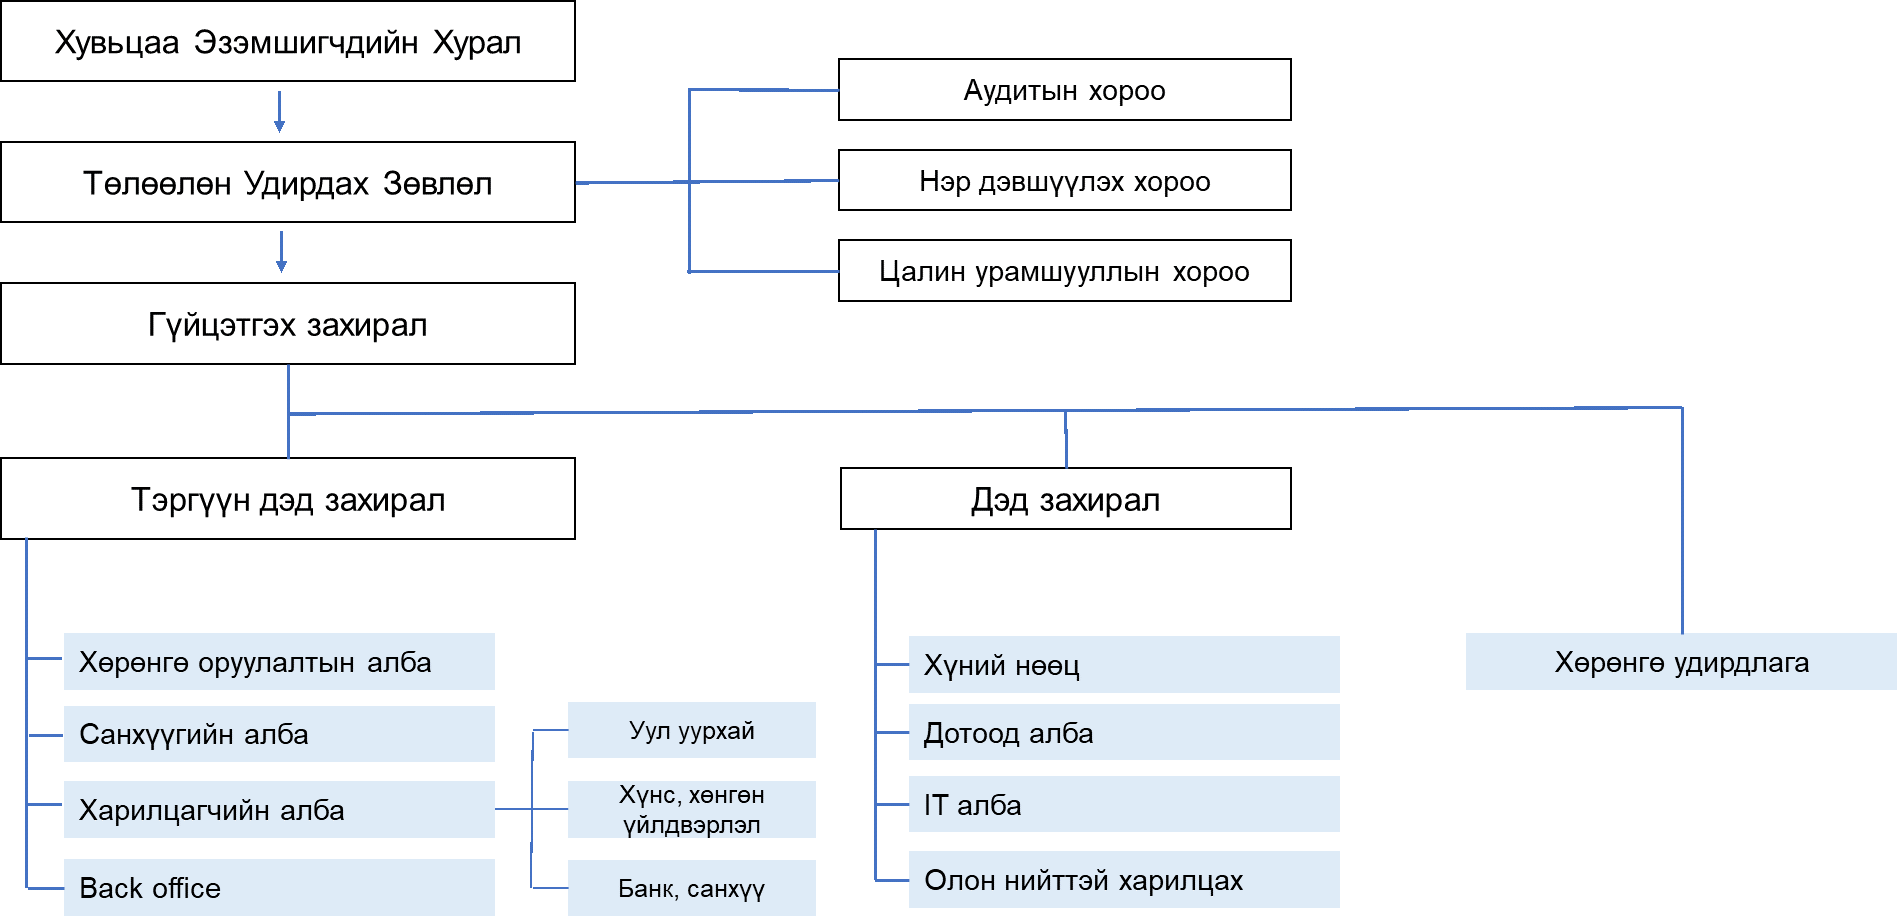
\includegraphics[scale=0.4]{assets/company-structure.png}
    \caption{БиДиСек бүтэц зохион байгуулалт}
    Ашигласан зургийн эх хувилбар\cite{company}
    % \label{fig:placeholder}
\end{figure}


